\documentclass[11pt,letterpaper]{article}
\usepackage{fullpage}
\usepackage[top=2cm, bottom=4.5cm, left=2.5cm, right=2.5cm]{geometry}
\usepackage{amsmath,amsfonts,amssymb}
\usepackage{lastpage}
\usepackage[inline]{enumitem}
\usepackage{fancyhdr}
\usepackage{mathrsfs}
\usepackage{xcolor}
\usepackage{graphicx}
\usepackage{hyperref}
\usepackage{subcaption}
\hypersetup{colorlinks=true, linkcolor=blue, linkbordercolor={0 0 1}}

\renewcommand{\arraystretch}{1.75}

\setlength{\parindent}{0.0in}
\setlength{\parskip}{0.05in}

\newcommand{\its}{\item[\tiny\textbullet]}

\pagestyle{fancyplain}
\lhead{Brad Cownden}
\chead{}
\rhead{June 18, 2020}
\cfoot{\small\thepage}
\headsep 36pt

\begin{document}
\vspace{.2in}
\begin{center}
    {\bf GPU Solutions for PSCAD: IT17112}
\end{center}

	\vspace{.25in}

\begin{tabular}{| p{0.2\textwidth} | p{0.75\textwidth} |}
	\hline
	Reporting Period & June 11, 2020 - June 18, 2020 \\ \hline

	Activities & \begin{enumerate*}
    \item[\tiny\textbullet] Ran a final check on self-consistency between two compilers of \emph{Province} data set.
    See figure~\ref{f:mhi_compare} for details. Observed that the relative differences
    between values of $\mathbf{x}$ over all time steps is small on average, but does contain some
    significant variation, while $\mathbf{b}$ demonstrated a much greater degree of variation. \newline
    \its Compiled and ran QRFactor on both NVIDIA \href{https://images.nvidia.com/content/tesla/pdf/nvidia-tesla-p100-PCIe-datasheet.pdf}{Tesla P100} 
    and NVIDIA \href{https://images.nvidia.com/content/technologies/volta/pdf/volta-v100-datasheet-update-us-1165301-r5.pdf}{V100 PCIe}.
    See table~\ref{t:gpu_stats} for a summary of hardware characteristics. \newline
    \its {\bf Best performance}: While the V100 card took approximately $9$ ms to perform the one-time factoring of the 
    full system matrix $A$, it provided an average solving time of $0.5$ ms per time step. With this timing, 
    the \emph{Province} data set could be solved for a million time steps in only 8.3 minutes. See figure~\ref{f:full_timings} for 
    a comparison of timings for various hardware.
    \end{enumerate*} \\ \hline

	Issues & \begin{enumerate*}
	\item[\tiny\textbullet] None
	\end{enumerate*} \\ \hline

	Milestones \newline Accomplished & \begin{enumerate*}
	\item[\tiny\textbullet] Ran QRFactor on Telsa P100 and V100 PCIe cards, and collected new timing data. \newline
    \its Significant per-time step speedup achieved on V100 hardware; average per-time step solve time $0.5ms$.
    \end{enumerate*} \\ \hline

	Milestones Not \newline Accomplished & \begin{enumerate*}
	\item[\tiny\textbullet] None
	\end{enumerate*} \\ \hline

	Next Week's \newline Milestones & \begin{enumerate*}
    \item[\tiny\textbullet] Discuss next steps.
	\end{enumerate*} \\ \hline

	Forwarded Issues & \begin{enumerate*}
	\item[\tiny\textbullet] None
	\end{enumerate*} \\ \hline
\end{tabular}


\begin{table}[b]
    \begin{tabular}{| c | c | c | c |}
        \hline
        {\bf NVIDIA GPU} & {\bf Compute Version} & {\bf CUDA Cores} & {\bf Double-Precision Performance} \\ \hline
        \href{https://www.nvidia.com/content/dam/en-zz/Solutions/design-visualization/documents/quadro-mobile-line-card-n18-11x8.5-r4-hr.pdf}{Quadro RTX 3000} & $7.5$ & $2304$ & $198.7$ GFLOPs \\ \hline
        \href{https://images.nvidia.com/content/tesla/pdf/nvidia-tesla-p100-PCIe-datasheet.pdf}{Tesla P100} & $6.0$ & $3584$ & $4.7$ TFLOPs \\ \hline
        \href{https://images.nvidia.com/content/technologies/volta/pdf/volta-v100-datasheet-update-us-1165301-r5.pdf}{V100 PCIe} & $7.0$ & $5120$ & $7.8$ TFLOPs \\ \hline
    \end{tabular}
    \caption{Short summary of hardware specifications for the three types of GPUs used. Links are to the 
    respective hardware datasheets.}
    \label{t:gpu_stats}
\end{table}


\begin{figure}[!ht]
    \centering
    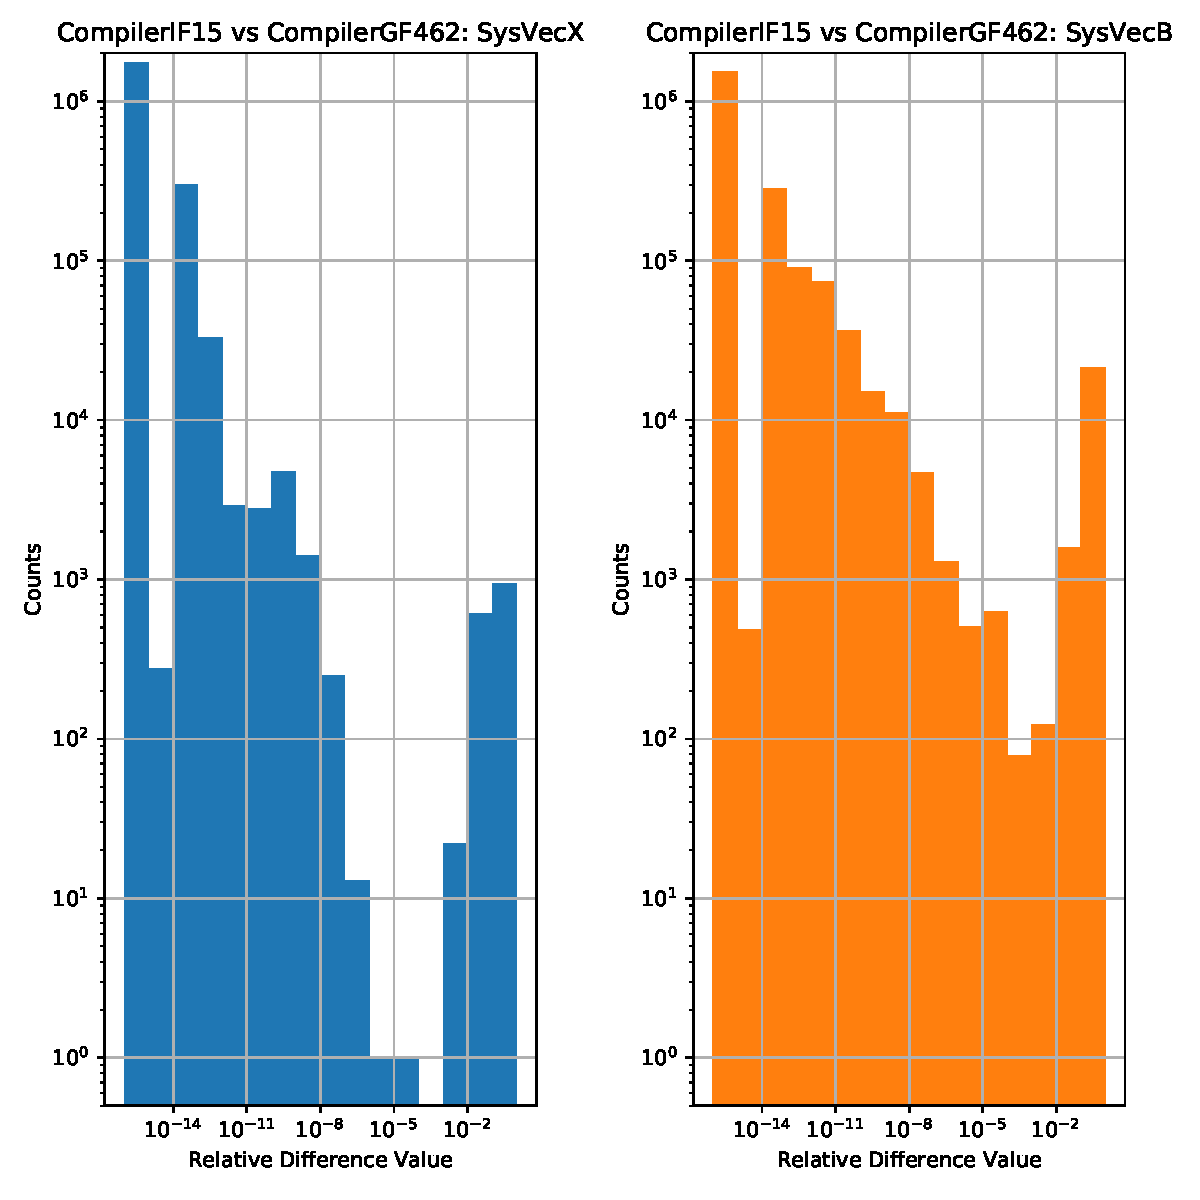
\includegraphics[width=\textwidth]{C:/Users/bradc/Documents/MHI/QRFactor/MHI_DirectCompare.pdf}
    \caption{\emph{Left} The relative difference between the full system output vectors $\mathbf{X}$ in 
    CompilerIF15 and CompilerGF462, over all time steps. \emph{Right} The same comparison, but applied 
    to full system input vectors $\mathbf{B}$.}
    \label{f:mhi_compare}
\end{figure}

\begin{figure}[!ht]
    \centering
    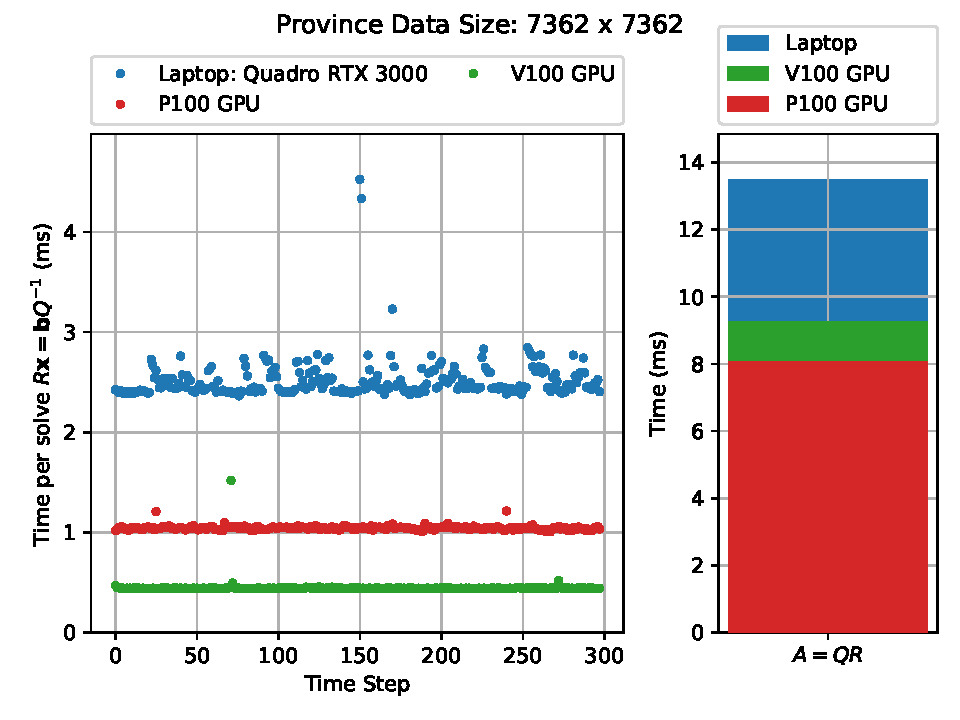
\includegraphics[width=\textwidth]{C:/Users/bradc/Documents/MHI/Output/FullTimings.pdf}
    \caption{\emph{Left} Time in milliseconds to solve the pre-factored system $R\mathbf{x} = \mathbf{b}Q^{-1}$ at each
    time step for the three hardware choices. \emph{Right} Time in milliseconds to perform the factoring of
    the full system matrix $A$ into $QR$ for each of the hardware choices. Note that while the V100 takes
    slightly longer to perform the one-time factoring of the matrix, it outperforms the other hardware 
    choices after the factoring is done.}
    \label{f:full_timings}
\end{figure}

\end{document}
